\documentclass[conference]{IEEEtran}
\usepackage{cite}
\usepackage{amsmath,amssymb,amsfonts}
\usepackage{graphicx}
\usepackage{textcomp}
\usepackage{xcolor}
\usepackage{multirow}
\usepackage{hyperref}
\usepackage{booktabs}
\usepackage{subcaption}
\usepackage{algorithm}
\usepackage{algpseudocode}

\DeclareMathOperator*{\argmin}{arg\,min}
\DeclareMathOperator*{\argmax}{arg\,max}
\DeclareMathOperator*{\minimise}{\textrm{minimise}}
\DeclareMathOperator*{\maximise}{\textrm{maximise}}
\newcommand{\Ie}{\textit{I.e.}\xspace}
\newcommand{\ie}{\textit{i.e.}\xspace}
\newcommand{\Eg}{\textit{E.g.}\xspace}
\newcommand{\eg}{\textit{e.g.}\xspace}
\newcommand{\probP}{\text{I\kern-0.15em P}}
\newcommand{\tl}[1]{\textit{[{\color{red}#1}]}}
\newcommand{\cm}[1]{\textit{{\color{blue}#1}}}
\newcommand{\erik}[1]{\textit{[{\color{brown}Erik: #1}]}}
\newcommand{\mr}[1]{\textit{[{\color{brown}Mohammed: #1}]}}
\begin{document}
\title{A Cloud Native Approach to Adversarial Robustness of Neural Networks}

\author{}
% author names and affiliations
% use a multiple column layout for up to three different
% affiliations
% \author{\IEEEauthorblockN{1\textsuperscript{st} Charles Meyers}
% \IEEEauthorblockA{\textit{Dept. of Computing Science} \\
% \textit{Umeå University}\\
% Umeå, Sweden \\
% cmeyers@cs.umu.se}
% \and
% \IEEEauthorblockN{2\textsuperscript{nd} Mohammad Reza}
% \IEEEauthorblockA{\textit{Elastisys} \\
% % \textit{Umeå University}\\
% % Lund, Sweden \\
% mohammad.saleh@elastisys.com}
% \and
% \IEEEauthorblockN{3\textsuperscript{rd} Tommy Löfstedt}
% \IEEEauthorblockA{\textit{Dept. of Computing Science} \\
% \textit{Umeå University}\\
% Umeå, Sweden \\
% tommy@cs.umu.se}
% \and
% \IEEEauthorblockN{4\textsuperscript{th} Erik Elmroth}
% \IEEEauthorblockA{\textit{Dept. of Computing Science} \\
% \textit{Umeå University}\\
% Umeå, Sweden \\
% elmroth@cs.umu.se}
% }

\maketitle


\begin{abstract}
Considering the growing prominence of production-level AI and the threat of adversarial attacks that can evade a model at run-time, evaluating the robustness of models to these evasion attacks is of critical importance.
Additionally, testing model changes likely means deploying the models to \textit{e.g.}, a car, a medical imaging device, or a drone to see how it affects performance, making un-tested changes a public problem that reduces development speed, increases cost of development, and makes it difficult (if not impossible) to parse cause from effect.
In this work, we used survival analysis as a cloud-native, time-efficient and precise method for predicting model performance in the presence of adversarial noise.
For neural networks in particular, the relationships between the learning rate, batch size, training time, convergence time, and deployment cost are highly complex, so researchers generally rely on benchmark datasets to assess the ability of a model to generalize beyond the training data. However, in practice, this means that each model configuration needs to be evaluated against real-world deployment samples which can be prohibitively expensive or time-consuming to collect --- especially when other parts of the software or hardware stack are developed in parallel. To address this, we propose using accelerated failure time models to measure the effect of hardware choice, batch size, number of epochs, and test-set accuracy by using adversarial attacks to induce failures on a reference model architecture before deploying the model to the real world. We evaluate several GPU types and use the Tree Parzen Estimator to maximize model robustness and minimize model run-time simultaneously. This provides a way to evaluate the model and optimise it in a single step, while simultaneously allowing us to model the effect of model parameters on training time, prediction time, and accuracy. Using this technique, we demonstrate that newer, more-powerful hardware does decrease the training time, but with a monetary and power cost that far outpaces the marginal gains in accuracy.
\end{abstract}

\begin{IEEEkeywords}
artificial intelligence, machine learning, adversarial AI, optimisation, compliance
\end{IEEEkeywords}


\section{Introduction}
\subsection{Motivation}
% \begin{itemize}
%     % \item \textit{BIG} Data is the trend
%     % \item Costs are astronomical
%     \item Prevailing regulatory framework is clear about the robustness requirements, documented software changes, and explainable processes.
%     \item Other work relies on unreliable test/train split methodology
%     \item Which means that cars, medical equipment is tested in the wild
% \end{itemize}

Recently, machine learning (ML) using deep neural networks has become a popular way to classify large amounts of data --- with applications ranging from medical imaging~\cite{ai_medical_imaging} to aviation~\cite{ai_aviation} and from security~\cite{ai_security,ai_luggage,ai_prison} to self-driving cars~\cite{ai_automotive}. 
Statistical learning theory~\cite{vcdimension} provides us no guarantees about the generalization performance of deep neural networks due to the massive number of tunable parameters. To overcome this, neural networks need large amounts of data~\cite{desislavov2021compute,bailly2022effects} to train ever-larger model~\cite{desislavov2021compute}, which has yielded increasingly marginal gains on test-set accuracy~\cite{sun2017revisiting}. It is also clear that reaching safety-critical standards using test-set accuracy would require an infeasibly large test set~\cite{meyers}. Therefore, we propose using accelerated failure time models to simulate edge-cases and verify models using a small number of samples.

\cm{
Modern neural networks are massive --- they have have grown to be one of the largest consumers of data-center power, especially with the rise of generative AI~\cite{msft_water}. For image systems, VGG19~\cite{vgg} is now considered small with \textit{only} 138 million parameters. ResNet152 has a similar number of parameters at 116 million~\cite{resnet}. However, modern advancements in transformer architectures have lead to an explosion in model size with the recent Mamba model boasting a massive 8 \textit{billion} tunable parameters~\cite{mamba}. At these scales, we have no statistical guarantees about the performance of these models and test-set validation would require many, many billions of samples for each and every model change.
}
% One of Facebook's large language models, dubbed LLaMA, was placed on the codesharing website, GitHub~\cite{llama}. Immediately, an open-sourced clone was created, which itself spawned hundreds of offshoot projects~\cite{openllama}. One version of this open-source large language model (LLM) was able to outperform the commercially available GPT-3.5 model~\cite{liu2023goat} with a fraction of the parameters (13 Billion), small enough to run on a laptop without a graphics processing unit (GPU), suggesting that consumer-level hardware can be used to effectively train large models in a reasonable time. Furthermore, popular models like Generative Pre-trained Transformer (GPT)~\cite{floridi2020gpt} or ResNet~\cite{resnet} have many millions or billions of parameters, requiring infeasibly large training datasets to verify a model\cite{vcdimension}. Media reports place the cost of training a GPT3 somewhere between 4 and 63 million dollars~\cite{Patel_Ahmad_2023,Feswing_2023}, meaning only a few entities in the whole world have the requisite hardware and/or cloud budget to build a competing system. While the benefits of a more portable model are plentiful, there is not yet a method for formalizing the relationship between cost and model performance.

Furthermore, even if we ignore the immense cost of training modern neural networks, the required number of test samples creates serious questions about the efficacy of the typical train/test split methodology for assessing model generalization~\cite{meyers} since regulatory standards around safety-critical software applications~\cite{IEC61508,iso26262,aviation_software,safetyframework} clearly define the maximum failure rate to be in the range $[10^{-12}, 10^{-15}]$ depending on the number of lives at risk. Furthermore, ensuring the robustness of ML models against adversarial noise has become a critical concern since inducing a failure at run-time has consistently shown to be trivial~\cite{adversarialpatch, carlini_towards_2017, croce_reliable_2020, hopskipjump, chakraborty2018adversarial, art2018}. Collecting, labelling, and testing a new set of data for every software change --- as required by law in most of the world~\cite{IEC61508,iso26262,aviation_software,safetyframework} --- would be prohibitively expensive for these large models. Therefore, a new evaluation methodology is required.

% As such, the methodology proposed in this paper, centered around survival analysis, tests a model against ``worst-case" (\textit{e.g.}, adversarial) inputs to verify the efficacy of one modelling deployment decision over another. 
We propose to use survival analysis as a methodological framework to model the failure conditions of a machine learning model. Instead of having a test set large enough to cover all of the failure cases, we generate adversarial samples crafted specifically to make the model fail and then use survival analysis to predict these failures in general.

In this work, we used accelerated failure-time methods to predict model performance as a function of various model parameters. The methodology outlined in Section~\ref{aft} allows the model-builder to minimize the training cost, optimise for adversarial robustness, estimate the effects of covariates on model performance during routine training procedures. Then, one can perform a cost analysis (Section~\ref{cost}). We then demonstrate the efficacy of this methodology in Section~\ref{results} by examining the role of hardware on model performance, the particulars of which are outlined in Section~\ref{experiments}.


\subsection{Contributions}
To tackle the problems of minimizing deployment cost while maximizing the model performance on both the test set and in the presence of adversarial noise we present a scalable and effective methodology (see Algorithm~\ref{fig:alg} and Figure~\ref{fig:experiments}) and software framework (see Figure~\ref{fig:architecture}) for the training (see Section~\ref{aft}) and evaluation (see Section~\ref{cost}) of machine learning models that:
\begin{itemize}
    \item Optimises for benign and adversarial accuracy simultaneously,
    % \item Extends survival analysis to the realm of neural networks, 
    \item Demonstrates a scalable and effective method to train a model while simultaneously estimating the effect of various hyperparameters, and
    \item Measures the power and monetary cost of deploying a model across different hardware architectures to model the trade-offs between deployment hardware and robustness.
    \item \cm{Demonstrates that, even when we control for the slower clock speed of "inference only hardware" compared to hardware marketed for training, that models trained using the "inference only" devices are more robust for image classification tasks than models built on hardware designed for training.}
\end{itemize}

Section~\ref{background} defines the terminology used throughout the paper. Section~\ref{aft} outlines the training and evaluation methodology presented in this paper.  Section ~\ref{cost} discusses the resulting cost analysis framework, arising from the methodology in the previous section. Section~\ref{experiments} outlines the software components and specific experiments that were conducted, while Section~\ref{results} contains the results and discussions of those experiments. Section~\ref{considerations} and Section~\ref{conclusion} reveal the caveats and the conclusions respectively.


\section{Background}
\label{background}



In this paper, we evaluate a comprehensive methodology for evaluating model robustness during training time and model the asymptotic effect of the various parameters in the hyper-parameter search space. For the sake of the reader, we provide a section for definitions and requisite background information below.


% Our experiments and analysis provide valuable insights into the trade-offs and considerations when deploying ML models under varying computational and adversarial constraints. 
\subsection{Cloud Architectures}


ML pipelines play a crucial role in the development and deployment of robust and accurate models. However, managing complex pipelines across diverse CPU and GPU architectures, ensuring robustness against adversarial attacks, and understanding the relationship between computational cost, model loss, and prediction accuracy remain ongoing challenges.
One popular solution is using a network of interconnected services~\cite{panchal2024reusable,hasselbring2017microservice,zhou2022online,singh2023load} where a \textit{service} is the smallest component of a ``cloud-native" software stack. In the context of ML, that might be some software component meant for training, inference, pre-processing, sampling, or any other arbitrarily small part of the data pipeline. 
A service \textit{mesh} typically consists of a set of interconnected components or proxies deployed alongside the services within the system.  These components facilitate various capabilities and functionalities essential for managing the communication between services. Kubernetes has become one of the largest open source projects on the code-sharing website Github~\cite{k8s-size} and provides a framework for managing, monitoring, and networking a self-scaling set of tools across arbitrary software and hardware architectures using a service mesh. For ML applications, these services are often divided into ``training" and ``inference" configurations that often have distinct hardware and software configurations~\cite{wang2019benchmarking}. In this work, we leveraged Kubernetes~\cite{k8s} to manage a multi-stage ML pipeline (see Figure~\ref{fig:experiments}) and measure the power and cost of training and evaluating the pipeline (see Figure~\ref{fig:architecture}) across a variety of different hardware architectures (see Table~\ref{tab:hardware}).


\subsection{ML Pipelines}
ML pipelines are often long-running and complex software tool-chains with many tunable hyperparameters. Managing, tracking, and controlling for various parameters is non trivial, but many management tools are available~\cite{dvc,hydra,k8s}. In general, a dataset is split into \textit{training} and \textit{test} sets. The training set is then used to determine the best configuration of a given model architecture on a given hardware architecture with the expectation that it will generalize both on the withheld test set and on new data generated and submitted by users. To verify the training process, the test set is validated against the \textit{inference} configuration of a model which may run on different hardware than the \textit{training} configuration to reduce cost, latency, or power consumption. Likewise, Nvidia offers hardware that is marketed as either for training (\textit{e.g.}, v100 and p100) or only for inference (\textit{e.g.}, l4).


\subsection{Classifiers}

We consider ML classifiers, $K(x; \theta)$ with model parameters, $\theta$. The true labels are denoted by $y$, and the model predictions by $\hat{y} = K(x; \theta)$ where $x$ is a mini-batch of size $N$ of data samples. The loss function, the measure of discrepancy between the true label and the predicted label, is denoted by $L(y, \hat{y})$.
Because of the complexity of modern machine learning models, researchers rely on numerical optimisation, and one popular choice of optimisation algorithm is \textit{stochastic gradient descent}, which updates the model parameters by taking a step in the negative gradient direction, where the gradient is computed using a subset (a mini-batch) of the training samples instead of all training samples.
% selects the next $N$ samples from the training set before adjusting the model parameters, $\theta$, in the direction that decreases the loss.
% This is in the direction of the negative gradient of the loss, $-\nabla L(y, K(x, \theta))$.
This procedure is repeated for some number of \textit{epochs} (iterations through the entire training set). Every iteration takes a step,
\begin{equation}
    \theta^{(i+1)} = \theta^{(i)} - \eta \nabla_{\theta^{(i)}} L(y, K(x, \theta^{(i)}))
    \label{eq:sgd}
\end{equation}
where the gradient is approximated using $b$ samples per mini-batch and $\eta$ is the \textit{learning rate} (or step size) that is tuned to the particular model and data.


\subsection{Learning Rate Selection}
\label{learning_rate}

Choosing a good learning rate is critical for model performance --- greatly effecting both the accuracy and the training cost. A small learning rate will more accurately approximate the class boundaries~\cite{cao2019generalization}, but will converge slower, all other things being equal. Of course `small` is arbitrarily defined, but the scale of the optimal learning rate will vary with \textit{e.g.}, the mini-batch size, number of epochs, dimensionality of the input data, \textit{etc.}~\cite{granziol2022learning}. GPUs with larger amounts of VRAM are able to hold more data in memory at a time, increasing the effective mini-batch size, and reducing the number of model-tuning steps per epoch. A ``good" learning rate will allow a model to converge quickly~\cite{smith2019super,granziol2022learning} and the ideal mini-batch size will be determined by the memory bandwidth of the GPU and the size of the model and the size and dimensionality of the data. However, since cloud infrastructure is virtualized and shared with other users, the available bandwidth will not necessarily match the peak available bandwidth specified by the manufacturer~\cite{sajid2013cloud}, so researchers must evaluate this \textit{in situ}. Furthermore, since hardware is typically billed by the hour on public clouds, optimising the training and inference times allows a model-builder to minimize the cost of deployment. 


\subsection{Adversarial Attacks}
\label{attacks}
In the context of ML, an adversarial attack refers to deliberate and malicious attempts to manipulate or exploit ML models. Adversarial attacks are designed to deceive or change the model's behavior by introducing carefully crafted input data that can cause the model to make incorrect predictions or otherwise produce undesired outputs. That is, a successful attack is one in which the model outputs on the original, unperturbed data, $\hat{y}$, are not the same as the model outputs on perturbed data, $\hat{y_a}$. That is \textit{adversarial success} or \textit{accelerated failure} is one in which
\begin{equation}
    \hat{y} \neq \hat{y_a} = K(x + \varepsilon; \theta).
\label{eq:adv_success}
\end{equation}
Additionally, one can measure the accuracy of the model when tasked with these adversarial samples, giving us a metric called \textit{adversarial accuracy} which is Eq.~\ref{eq:acc} calculated on the perturbed samples. The goal of an adversarial attack is often to exploit vulnerabilities in the model's decision-making process or to probe its weaknesses. These attacks can occur during various stages of the ML pipeline, including during training~\cite{biggio_poisoning_2013, saha2020hidden}, inference~\cite{chakraborty_adversarial_2018, orekondy2019knockoff}, or deployment~\cite{chakraborty_adversarial_2018, choquette2021label, li2021membership, carlini_towards_2017, adversarialpatch, pixelattack, hopskipjump}.

% \cm{I cut itemized list more discussion about learning rate tuning?}
% \begin{itemize}
%     \item Evasion Attacks: These attacks aim to manipulate input data during the inference phase to deceive the model into misclassifying certain inputs or otherwise change the behavior of a modelt~\cite{ carlini_towards_2017, adversarialpatch, pixelattack, hopskipjump}.
%     \item Poisoning Attacks: In poisoning attacks, the attacker intentionally injects malicious or manipulated training samples into the training dataset to influence the model's behaviour at run-time~\cite{biggio_poisoning_2013, saha2020hidden}. 
%     \item Inference Attacks: These attacks exploit the model's output or responses to obtain sensitive information about the training data or other confidential details~\cite{chakraborty_adversarial_2018, orekondy2019knockoff}.
%     \item Model Inversion Attacks: Model inversion attacks aim to infer sensitive information about the training data or proprietary model by exploiting the model's outputs~\cite{chakraborty_adversarial_2018, choquette2021label, li2021membership}. 
% \end{itemize}

One of many possible attacks is designed to induce failures as quickly as possible, and is  conveniently called the \textit{fast gradient method}~\cite{fgm}. It works by applying noise to a set of samples, $x$, to generate adversarial examples, $x_a$, such that,
\begin{equation}
x_a = x + \eta \cdot \mathrm{sign}(\nabla_x L(y, K(x, \theta))).
\label{eq:fgm}
\end{equation}
In essence, this is process seeks to increase the loss by changing the input data, in contrast to model training which seeks to minimize the loss by changing the model parameters.


\subsection{Adversarial Analysis}

In the case of safety- or security-critical domains, considering the worst-case scenario is routine~\cite{sajid2013cloud}. Whether in the context of automotive safety~\cite{ai_automotive}, crytographic systems~\cite{leurent2020sha,kamal2017study}, or healthcare malpractice~\cite{ai_medical_imaging}, a component, algorithm, or system is considered broken if the \textit{failure rate} exceeds a certain amount, depending the risk to human life~\cite{IEC61508}. An order of magnitude more automotive accidents, security breaches, or deaths due to negligence would be unacceptable and, as such, these standards are non-negotiable. However, this would mean testing many millions of samples for every model change that has the potential to injure a human, with orders of magnitude more stringent requirement in the case of potentially fatal systems. This is just not computationally feasible. Instead, researchers can use adversarial failure analysis~\cite{carlini_towards_2017,biggio_evasion_2013,meyers} to improve the precision of our estimates while only using a small set of test-data.





\section{Survival Analysis for Robustness Verification during Training}
\label{aft}

We propose a methodology for model training and verification using accelerated failure-time (AFT) models, drawn from the field of \textit{survival analysis}, with a focus on cost-efficient evaluation methods.
AFT models are statistical models used to analyze multivariate effects on the observed failure rate to predict the time-to-failure across a wide variety of circumstances~\cite{aft_models,kleinbaum1996survival}. In medical science, these models are used to make claims like ``smokers are twice as likely to die from lung cancer'' or used to set the operating limits of manufactured components. This methodology can be used to map the relationship between various model tuning parameters and their effect on model performance.
The next section outlines the methodology for modelling the effect of model hyper-parameters during routine training procedures. We precisely outline the methodology for using survival analysis during the training of machine learning methods. 
% First, we present the proposed procedure in Algorithm~\ref{fig:alg} and a visual diagram of it in Figure~\ref{fig:experiments}. Then, in the sections below, we define accuracy (Section~\ref{acc}) and failure rate (Section~\ref{failure_rate}) in the context of survival analysis to make the concept of survival time clear (Section~\ref{survival_time}). We then discuss the importance of the ``acceleration assumption" (Section~\ref{accelerated}), the optimisation algorithm (Section~\ref{optimisation}), and the advantages of this approach (Section~\ref{advantages}).


\begin{algorithm}[h!]
    \caption{Survival Analysis for ML}
    \label{fig:alg}
\begin{algorithmic}
    \Require Samples $x$ of size $N$, model parameters $\theta$, loss function $L(y, \hat{y})$, classifier $K(x; \theta)$, and the number of trials, $n$, where the subscripts $t,i,a$ refer to the respective value for either the train, test, and/or attack sets, \textit{e.g.}, $N_t$ is size of the training set.
    \State Initialize classifier $K(x, \theta)$, training/inference/attack generation time arrays $T_t/T_i/T_a$, benign/adversarial accuracy arrays, $\lambda_{ben}/ \lambda_{adv}$
    \State $i = 0$
    \While{ $i < n$}
    \State \textbf{Initialize:} Random State, $R$ and split the classification data into the training set $x_t$ and the inference set $x_i$.
    \State \textbf{Optimise $L(y, \hat{y})$:} over $x_t, \theta$ according to some method (e.g Eq.~\ref{eq:sgd}) with a given batch size, $b$, and number of epochs, $m$.
    \State  $T_t[i] \gets$ Training Time.
    \State  $ \hat{y_i} = K(x_i, \theta) $.
    \State  $ T_i[i] \gets $  Inference Time.
    \State  $\lambda_{ben}[i] \gets $  Benign Accuracy (Eq.~\ref{eq:acc}).
    \State find $x_a$ with Eq.~\ref{eq:fgm}.
    \State  $T_a[i] \gets$ attack generation time.
    \State  $ \hat{y}_a = K(x_a, \theta) $.
    \State  $\lambda_{adv}[i] \gets $  Adversarial Accuracy (Eq.~\ref{eq:acc})
    \EndWhile
    \State $S_{\theta}(T_a) \approx \phi N_a \cdot \lambda_{adv}$ with $\lambda_{ben}$, $T_t$, $T_i$, $m$, $b$, $R$ \\
    % used as covariates to some acceleration factor, $\phi$ and  $N_a$ is the attack size array.
    \Return $S_{\theta}$
\end{algorithmic}
\end{algorithm}


\begin{figure}
    \centering
    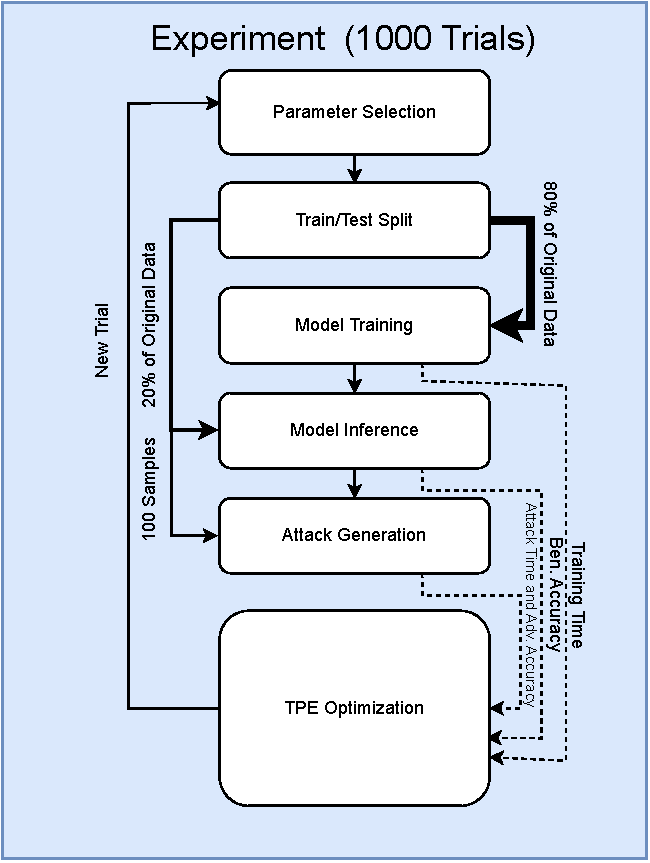
\includegraphics[width=.35\textwidth]{plots/experiment.pdf}
    \caption{Experimental Pipeline Diagram}
    \label{fig:experiments}
\end{figure}



\subsection{Accuracy}
\label{acc}

Accuracy measures the vulnerability or susceptibility of the model to failures. A larger accurate indicates a higher rate of true classifications, signifying a weaker model in terms of \textit{robustness} against (noise-induced) failures. Throughout, we use the terminology \textit{benign} accuracy to refer to the performance on the test set using unperturbed data and \textit{adversarial} to refer to the performance in the presence of additive noise that is intended to confuse the model. The subscripts \textit{ben} and \textit{adv} are used respectively. The accuracy, $\lambda$, is defined as
\begin{equation}
    \lambda:= \mathrm{Accuracy} := 1 - \frac{\mathrm{False~Classifications}}{\mathrm{Total~Classifciations}},
    \label{eq:acc}
\end{equation}
which is generally assumed to indicate the rate of successes in real-world data sampled from the same distribution as the training data~\cite{tan2021critical}. However, the normal test/train split methodology consistently overestimates the model's performance in the presence of adversarial noise~\cite{croce_reliable_2020.
In addition, it ignores the run-time cost of a given architectural decision, caring only about accuracy on benchmark data~\cite{desislavov2021compute,bailly2022effects}. Additionally, it has been shown that it is trivial to generate adversarial counter examples that reveal the test/train split methodology to be optimistic at best~\cite{carlini_towards_2017,adversarialpatch,pixelattack,hopskipjump,biggio_poisoning_2013,chakraborty_adversarial_2018,dohmatob_generalized_2019,meyers}. 


\subsection{Failure Rate}
\label{failure_rate}

The failure rate refers to the percentage or proportion of examples that cause the targeted ML model to misclassify or produce incorrect outputs~\cite{meyers}. To encompass the cost of a particular model or attack, the proposed methodology considers failures to be a function over some time interval (\textit{e.g.}, training time, inference time, attack generation time, \textit{etc.}) and some covariates, $\theta$, so that the failure rate is the average time until a failure in a time interval around time, $t$, such that:
\[
    h_{\theta}(t) :=  \frac{p(\textrm{False~Classification} \mid \theta)}{\Delta t} t,
\]
where $p(\textrm{False~Classification} \mid \theta)$ is the probability of a false classification given a particular set of hyper-parameters, $\theta$, $\Delta t$ is a time interval, and $t$ is a point in time.  Note that  $1 - \lambda$  is an estimate of this value when $\Delta t = t$ and converges to this value as the number of samples, $N \rightarrow \infty$. By modelling accuracy as a function of time, one can then compare the probability of failure to the cost, which is also measured in time, allowing one to make deployment decisions based on the risk analysis standards outlined in IEC61508~\cite{IEC61508}. This then allows us to make claims like ``increasing training time by X\% will yield survival time gains of Y\%''~\cite{meyers_aft}.


\subsection{AFT Models}
\label{survival_time}

AFT models are widely used in industrial, medical, or risk-mitigation contexts~\cite{kleinbaum1996survival, aft_models} to model the effect of covariates on a model's expected time-to-failure (also called survival time. For industrial components, this often means testing the component under a variety  of extreme circumstances to induce failures prematurely. For medical applications, this is used to model the effect of demographic characteristics or the efficacy of certain treatments on a given disease. For machine learning, this means inducing failures during training to measure generalization performance.

The point of this is to model the \textit{survival time}, $S_{\theta}(t)$, as a function of the time, $t$,  and some set of model parameters, $\theta$ such that,
$$
    S_{\theta}(t) = p(T>t) = \exp\left(-\int_0^t h_{\theta}(u) \, du\right)
$$
where $p(T>t)$ is the probability that a model has not failed by time $t$ (``survives'' beyond time $t$). The expected survival time is
\[
	\mathbb{E}_{S_\theta}[T] = \int_0^{t^*}  S_\theta(t) \,dt,
\]
where $t^*$ is the latest time observed in the survival data. However, modelling $S_{\theta}(t)$ requires a choice in modelling function for $S_{\theta}$. The Log-Logistic, Log-Normal, and Weibull functions are widely used alternatives~\cite{kleinbaum1996survival}. For each trial, one can measure the inference time to define the time interval and the accuracy to estimate the number of failures in that time interval. The full algorithm can be seen in Algorithm~\ref{fig:alg}.


\subsubsection{Choosing the best AFT Model}

To choose a best-fit from the possible AFT functions, one should prepare the collected metrics and scores and then compare them using \textit{e.g.}, Akaike Information Criterion (AIC), Bayesian Information Criteria (BIC), or Concordance, as per the best-practices for this methodology~\cite{aft_models,kleinbaum1996survival}. For AIC and BIC, that means choosing the smallest value. Concordance, however, is a number between $0$ and $1$ that quantifies the degree to which the survival time is explained by the model, where a $1$ reflects a perfect explanation~\cite{kleinbaum1996survival} and 0.5 reflects random chance. By evaluating $\mathbb{E}_{S_\theta}[T]$ under extreme perturbations, one can test the model and minimize the number of evaluated samples~\cite{aft_models,kleinbaum1996survival} rather than relying on the $> 10^{12}$ samples as required by IEC61508~\cite{IEC61508}. We also noted the integrated calibration index (ICI) as well as the error at the median (E50)~\cite{ici}. These are the mean absolute difference between observed and predicted probabilities and the median absolute difference between observed and predicted probabilities, respectively~\cite{ici}. Then, the fitted AFT models were plotted using that compares the fitted AFT model to a cubic spline fit to the data~\textit{et al.}~\cite{ici}  to visually inspect each model for goodness-of-fit (see Figure~\ref{fig:qq}). \cm{Additionally, the data were split into a training set that was used to fit the model (80\%) and an unseen test set (20\%) and the concordance, ICI, and E50 were measured for both.}



\subsection{Benign and Adversarial Survival Time}
\label{accelerated}

Using accelerated failure time models under adverse ones (accelerated failure time), $S_{adv}$. The survival time for is
$$
    S_{adv} := S(t_i; x, y, \theta) \mathrm{~~where~~} 0 < \varepsilon \leq \varepsilon_{max}.
$$
This can also be thought of in terms of the accelerated failure time assumption~\cite{kleinbaum1996survival}
\begin{equation} \label{assumption}
    S_\theta(t) = S_0 \left( \frac{t}{\phi_\theta(x)} \right)
\end{equation}
where $\phi$ is some acceleration factor described by the joint effect of the covariates and $S_0$ is the baseline hazard function (where the effect of the covariates are 0). This assumption means we can evaluate the generalization performance using a small number of adversarial samples~\cite{kleinbaum1996survival}, with our precision coming from careful time measurements rather than massive test sets.
However, in order to find the optimal hyper-parameter configurations for both the model and attack, one must search this space systematically.


\subsection{Optimisation}
\label{optimisation}

ML models are typically trained by examining the effect of the entire hyper-parameter space on the resulting accuracy. However, the number of hyper-parameter combinations are often infinite or at least exponential in the number of hyper-parameters,
making it infeasible to exhaustively evaluate the entire hyper-parameter search space. Additionally, the goals of test-set accuracy and adversarial accuracy are often at odds~\cite{carlini_towards_2017} --- with several researchers noting an inverse relationship between model accuracy and model robustness~\cite{carlini_towards_2017,meyers,dohmatob_generalized_2019}. Therefore, a proper search would keep this dual-objective in mind.
To optimise for adversarial and benign accuracy simultaneously, we propose the use of the Tree-structure Parzen Estimator (TPE) because it has been shown to converge  over tens or hundreds of trials rather the the 1000s of trials required by other multi-objective optimization algorithms like CMAES or NGSA-II~\cite{ozaki2020multiobjective,optuna,tpe_params}.




\section{Cost Analysis}
\label{cost}

In addition to the survival analysis, we can use an estimate of survival time to conduct a cost analysis as dictated by IEC61508~\cite{IEC61508} which allows us to quantify the marginal risk. To quantify this marginal risk, one must measure the benign and adversarial accuracies (see Eqs.~\ref{eq:adv_success}~and~~\ref{eq:acc}), the model training time ($t_{t}$), the model inference time or latency ($t_{i}$), the attack generation time ($t_{a}$), the cost per hour for a particular hardware ($C$), as well as the power consumption ($P$) of each tested model and attack. 


\subsection{Accuracy}

In order to estimate the number of failures in a given time period, we measured both the benign accuracy and the adversarial accuracy, which reflect the normal test-set accuracy and the test-set accuracy in the presence of additive noise in the direction that maximizes loss. Under the AFT framework above, we can use the adversarial accuracy as a measure of the survival time across a specified time period as outlined in Algorithm~\ref{fig:alg}.


\subsection{Training Time}

The training time, $T_t$, is the time it takes to evaluate $n$ samples when $t_t$ is the training time per sample. It is defined as
$$
    T_t := t_t \cdot n  \cdot m,
$$
where $m$ is the number of epochs.


\subsection{Latency}

Latency is the time it takes to respond to a query. We assume that latency per sample is
$$
    T_i := t_i \cdot n,
$$
which will be driven by the memory bandwidth (measured in bits/second) of a given CPU or GPU and the size~\cite{vgg} and complexity~\cite{resnet} of a given neural network architecture.


\subsection{Attack Generation Time}

A successful attack is one that induces failure in a model. That is, the expected survival time, $\mathbb{E}_{S_\theta}[T]$, can be thought of as the average time it takes for an attacker to induce a change in the model output. We approximate this for each attack/defence configuration by the total attack time, $T_a$, for $n$ samples, $i$ iterations, and attack time per sample, $t_a$, as
\begin{equation}
    \label{attack_time}
    T_a := t_a \cdot n \cdot i.
\end{equation}
In the interest of time, our chosen attack, FGM, uses only a single iteration $i =1$~\cite{fgm}.


\subsection{Cost}

Furthermore, we approach the cost of deployment at two scales. Firstly, we consider the cloud-rental scale, where a small-business might test and deploy a model using \textit{e.g.}, the Google Cloud Platform\footnote{\href{https://cloud.google.com}{https://cloud.google.com}} (GCP) compute costs as a measure of total cost. However, at a certain scale or with certain applications, it is  more appropriate to talk about cost in terms of power (\textit{e.g.}, to deploy a self-driving car with a useful operating range). Finally, we define best-case and worst-case success metrics that provide an efficient way to minimize the latency, cost of deployment, and 
maximize the generalized performance of a model. We define the training cost as
$$
    C_t = C_h \cdot T_t,
$$
the cost of model inference time as,
$$
    C_i = C_h \cdot T_i,
$$
and the cost of an attack as,
$$
    C_a = C_h \cdot T_a.
$$
where $C_h$ is the cost per unit time for the hardware, $T_t$ is the training time, $T_i$ is the inference time, and $T_a$ is the attack generation time, as defined above.


\subsubsection{Power}

The power consumption for a particular piece of hardware, $P_h$, measured in Watts (Joules per second), can be thought of similarly such that the total power consumption of model training is
$$
    P_t = P_h \cdot T_t,
    \label{eq:power_training}
$$
the power consumption during model inference is
$$
    P_i = P_h \cdot T_i,
    \label{eq:power_inference}
$$
and the power consumption during attack generation is
$$
    P_a = P_h \cdot T_a,
    \label{eq:power_attack}
$$
where $P_h$ is the cost per unit time for the hardware, $T_t$ is the training time, $T_i$ is the inference time, and $T_a$ is the attack generation time, as defined above.


\subsection{Why Cost Matters}

In security analysis, it is  routine to think in optimistic terms for both the attacker and defender. In cryptography, these ideal attack- and defence-scenarios are used to test the computational feasibility of subverting a particular cryptographic system~\cite{kamal2017study,leurent2020sha} (\textit{e.g.}, whether or not a given cryptographic method should be considered ``broken"). Using AFTs, one can model the Pareto front --- the set of points that are superior to all others in the search space --- of either party~\cite{zitzler2008quality}. By using a whitebox attack to generate the failures, we ensure that our defender operates under the worst case scenario while the attacker operates under their best case scenario to yield a worst-case failure rate. As such, we center our analysis on the whitebox Fast Gradient Method~\cite{fgm} (see Eq.~\ref{eq:fgm}) which is both effective and fast~\cite{meyers}. If the cost to a model builder is much larger than the cost to an attacker ($C_t \gg C_a$), then it is  clear that the model is ``broken" in this cryptographic sense and can be discarded as ineffective. 


\section{Experiments}
\label{experiments}

This section outlines specific implementation details for the evaluation of the survival analysis methodology outlined in Section~\ref{aft} and the cost analysis methodology outlined in Sec~\ref{cost}.


\subsection{Cloud Platform and Hardware}
To conduct the experiments and have access to different types of hardware, we utilized GCP. Six virtual machines running container optimised operating system provided by GCP constituted the test-bed. Using Google Kubernetes Engine 1.27.3 and Containerd 1.7.0, a cluster consisting of six worker nodes was created. Three worker nodes were responsible for running the monitoring platforms-- Prometheus 2.47.2 and Grafana 10.2.0. These nodes were of the ``e2-medium" instance type provided by GCP. In total, three GPU architectures were used--the Nvidia P100, V100, and L4. For P100 and V100 GPUs, the ``n1-standard-2'' type was used for the nodes and for L4 GPUs the ``g2-standard-4'' was used.

To assess the energy consumption of the experiments deployed on a Google Kubernetes Engine, the Kubernetes Efficient Power Level Exporter (KEPLER) was employed as measurement tool~\cite{amaral2023kepler}. This approach enables gathering energy consumption data on granular levels as it runs in Kubernetes cluster and capable of collecting energy consumption of Kubernetes components. In essence, KEPLER uses extended Berkeley Packet Filter (eBPF) to probe energy-related system stats and exports them as Prometheus metrics. The eBPF can be described as a lightweight and sandboxed virtual machine (VM) in kernel space. The eBPF programs are invoked by the kernel when certain events occur. Examples of such events include system calls or network activity. These processes enable deep analysis and full control over different events with low overhead~\cite{sedghpour@ebpf}. A diagram of the cloud architecture can be found in Figure~\ref{fig:architecture}. Finally, for a cost-effective model evaluation technique, all of the experiments were restricted to a single one-thousand United States dollar budget (a research grant from Google). Approximately 10\% of this was used for development and 90\% was used for the evaluations.

\begin{figure*}
    \centering
    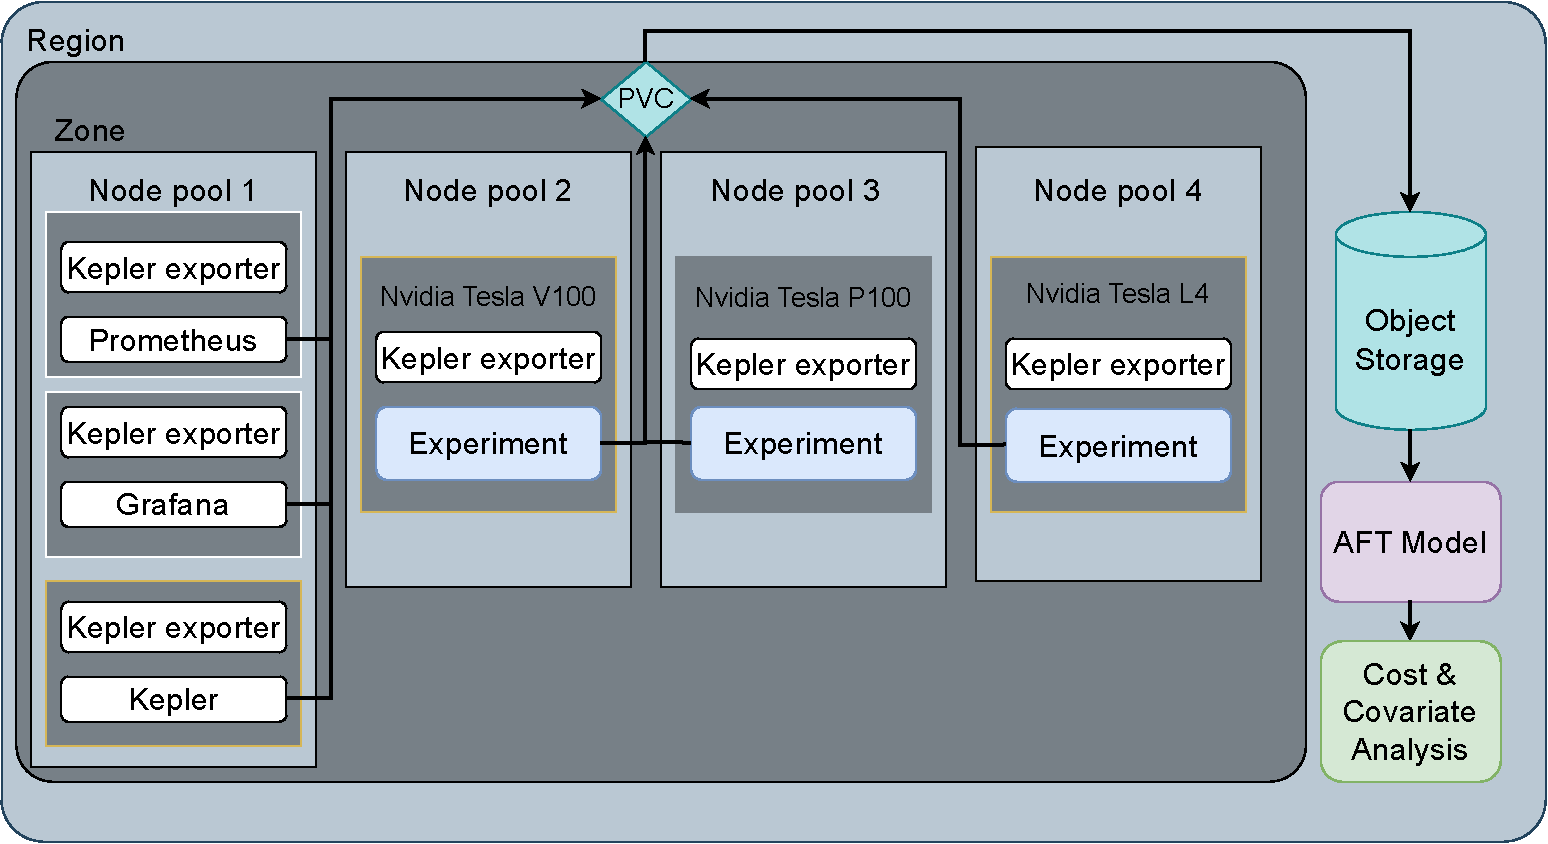
\includegraphics[width=.8\textwidth]{plots/architecture.pdf}
    \caption{Cloud Architecture Diagram}
    \label{fig:architecture}
\end{figure*}


\subsection{AFT Models}

For each hardware configuration and dataset, the TPE algorithm was used to select the hyper-parameters~\cite{ozaki2020multiobjective,zitzler2008quality}, and it was iterated for 1000 trials. This was chosen to be significantly larger than the 200 used successfully by Watanabe~\textit{et. al.}~\cite{tpe_params} while still allowing for reasonable run times. In reality, the correct number of iterations will be determined by the frequency of local minima across the search space and the number of optimisation criteria where marginally more minima or criteria require significantly more trials to yield accurate results~\cite{legriel2010approximating}. Examining the effect of this and other TPE parameters on the total run-time and performance of this methodology was outside the scope of this work.
We used three optimisation criteria: benign accuracy, training time, and adversarial accuracy, seeking to maximize both benign and adversarial accuracy while minimizing training time (and therefore deployment cost). We selected a set of parameters as per the TPE algorithm and trained on 80\% of the samples for each of the MNIST, CIFAR10, and CIFAR100 datasets. Of the remaining samples, 100 were withheld to be attacked and used to evaluate the adversarial accuracy. Figure~\ref{fig:experiments} illustrates this methodology. For each dataset, we tested this on ten random splits of the data to create 10 unique test/train pairs. For each trial, we recorded attack generation time, model training time, model inference time, benign accuracy and adversarial accuracy, and the size of the training set, test set, and attack set. Using these values, we fit an AFT model to the number of failures (indicated by accuracy and sample size) and the attack generation time after adding dummy variables for the dataset and hardware device. Additionally, we approximate the AFT model using the methodology described in Algorithm~\ref{fig:alg}.


\subsection{Datasets}

The AFT models were evaluated using the MNIST~\cite{mnist}, CIFAR10\cite{cifar}, and CIFAR100\cite{cifar} datasets, chosen primarily for their standardized use in adversarial analysis~\cite{madry2017towards,croce_reliable_2020,carlini_towards_2017,deepfool} and decades of experimental results.
Before training, we centered and scaled the data so that the attack distance would be analogous for all tested datasets. Furthermore, to reduce the complexities of system overhead, distributed or federated training, and the effect of shared cloud environments, we restricted ourselves to datasets that were small enough to reside entirely within GPU memory with the model, since the disk read speed in cloud environments is incredibly variable.


\subsection{Models}

The evaluations were restricted to a single model. Primarily, this was done to meet the budgetary constraints since evaluating more models would mean evaluating fewer pieces of hardware. As discussed in Section~\ref{learning_rate}, the relationship between hardware specifications, hyper-parameters, and performance is highly complex and hard to predict. So, we sampled learning rates $\in [10^{-6}, 1]$, batch sizes $\in [1, 10^5]$, and epochs $\in [1, 50]$ for MNIST and CIFAR10 on the P100 and V100. For CIFAR100, the range of the tested epochs was increased to be $\in [1, 100]$. The Feature Squeezing defence~\cite{feature_squeezing} was used to evaluate the efficacy of different bit-depths on the L4 hardware, as provided by IBM's adversarial robustness toolbox~\cite{art2018} with bit depths $\in [4,8,16,32,64]$ which casts the inputs into \texttt{pytorch} compatible arrays. Model parameters were chosen using the \texttt{optuna} optimisation framework, the configuration was handled by \texttt{hydra}, and \texttt{dvc} was used to ensure reproducibility and aid in collaborative development.


\subsection{Attacks}

To examine the effect of model parameters at run-time, evasion attacks, which attack the model at the prediction stage, were examined. Prior research~\cite{meyers,meyers_aft} has shown that the Fast Gradient method (see Eq.~\ref{eq:fgm}) is consistently the most effective at inducing a large number of failures in a small amount of time. To evaluate the effect of adversarial noise on the samples, the noise levels were varied $\varepsilon \in (0, 1]$. This was done using the \texttt{adversarial-robustness-toolbox} package maintained by a team at IBM~\cite{art2018}.


\subsection{GPU Configurations}

Several hardware configurations were tested, that had various hourly costs, peak power demands, and theoretical memory bandwidths. The V100 was chosen as a baseline, since it is routinely used in the literature~\cite{svedin2021benchmarking,xu2018deep}. The P100 architecture comes from the same line of server-grade GPUs, but from an older generation. The L4, however, is advertised as a machine built for inference --- not training --- relying on a smaller number of bits per tensor core. Consequently, the number of operations per second depends on the bit depth of the data and model weights, with peak numbers outlined in Table~\ref{tab:hardware} for 8-bit inputs. The rental cost of the hardware, measured in United States Dollars per hour, indicates the operating cost of a given model. To calculate this, the price per hour from each cloud service pricing page\footnote{Google Cloud prices for P100 and V100 obtained \href{https://cloud.google.com/compute/gpus-pricing}{here.} Google Cloud prices for L4 obtained \href{https://cloud.google.com/compute/vm-instance-pricing\#accelerator-optimised}{here.}} were used and the cost of training ($C_{t}$) and the cost of inference ($C_{i}$) calculated from the cost of hardware ($C_{h}$), the training time ($T_{t}$), and the inference time ($T_{i}$).
\begin{table}[h]
    \centering
    \begin{tabular}{lllll}
    \toprule
                            & V100   & P100   & L4    &  \\
    \midrule
    Cost (USD/hour)         & 2.55   & 1.60   & 0.81   &  \\
    Power (Watts)           & 250    & 250    & 72    &  \\
    Memory Bandwidth (GB/s) & 900    & 732    & 300   &  \\
    \bottomrule
    \end{tabular}
    \caption{Hardware specifications for the tested GPUs. The specifications were retrieved from Nvidia's website at the following links: 
    \href{https://images.nvidia.com/content/technologies/volta/pdf/volta-v100-datasheet-update-us-1165301-r5.pdf}{V100 Datasheet},
    \href{https://images.nvidia.com/content/tesla/pdf/nvidia-tesla-p100-PCIe-datasheet.pdf}{P100 Datasheet}, and
    \href{https://nvdam.widen.net/s/rvq98gbwsw/l4-datasheet-2595652}{L4 Datasheet}. Prices were retrieved from Google Cloud Platform for the \texttt{europe-west4} region on 3 December 2023 at \href{https://cloud.google.com/pricing/list}{this link}.
    }
    \label{tab:hardware}
\end{table}


\subsection{Survival Analysis}

In addition to the optimisation criteria of benign/adversarial accuracy and training time, prediction times, attack times, power consumption, batch size, and number of epochs were also collected to be used as covariates in the AFT model, $S_{\theta}(t)$. To fit the AFT model and to plot the effect of the covariates, the \texttt{lifelines} Python package was used~\cite{lifelines}. The Weibull, Log Logistic, and Log Normal AFT models (see Section~\ref{aft}) were also compared. 


\section{Results and Discussion}
\label{results}

This section presents and discusses the results for all of the experiments across all datasets and hardware. First, the accuracy, training time, inference, and monetary cost are discussed in Secs.~\ref{res:acc}-\ref{res:cost}, followed by the fitted AFT model in Section~\ref{res:aft}.


\subsection{Accuracy}
\label{res:acc}

Figure~\ref{fig:acc} shows the benign (left) and adversarial (right) accuracies for all datasets and hardware. It demonstrates little to no change in accuracy or adversarial accuracy, regardless of hardware. The benign accuracy decreases with difficulty (CIFAR10 vs MNIST) or with the number of classes (CIFAR10 vs CIFAR100). For all three datasets, the adversarial accuracy becomes the reciprocal of the number of classes (\textit{i.e.}, the accuracy we would expect with random data), demonstrating the efficacy of the attack outlined in Section~\ref{optimisation}.

\begin{figure}[h!]
    \centering
    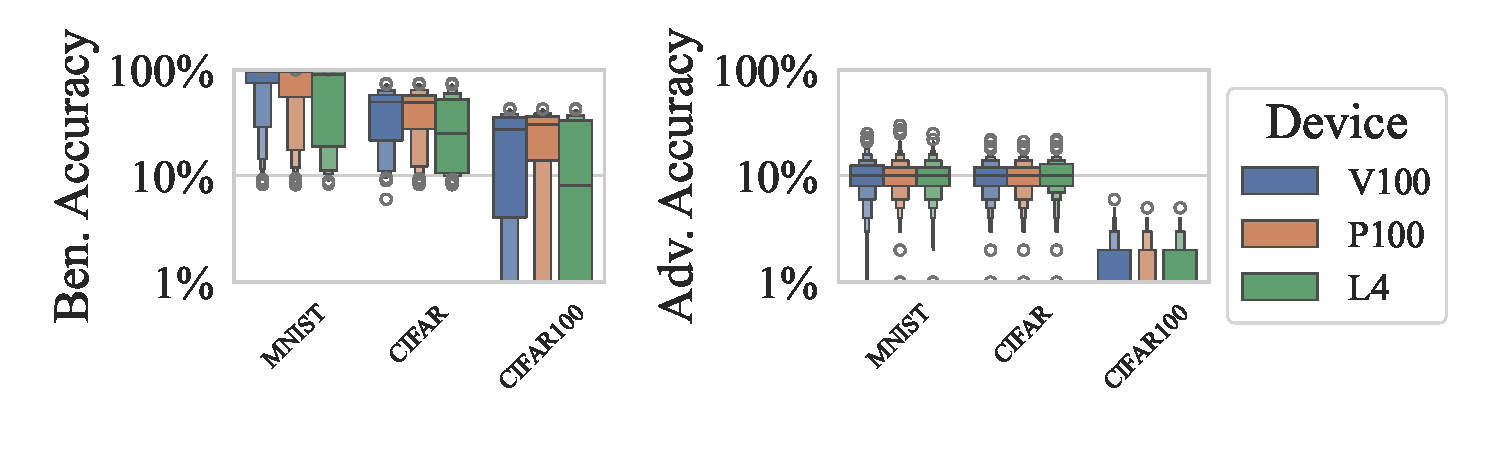
\includegraphics[width=0.5\textwidth,clip]{plots/combined/acc.pdf}
    \caption{Ben. and Adv. Accuracy Across Datasets and Hardware.}
    \label{fig:acc}
\end{figure}

\begin{figure*}[h]
    \centering
    \begin{subfigure}[b]{.8\textwidth}
        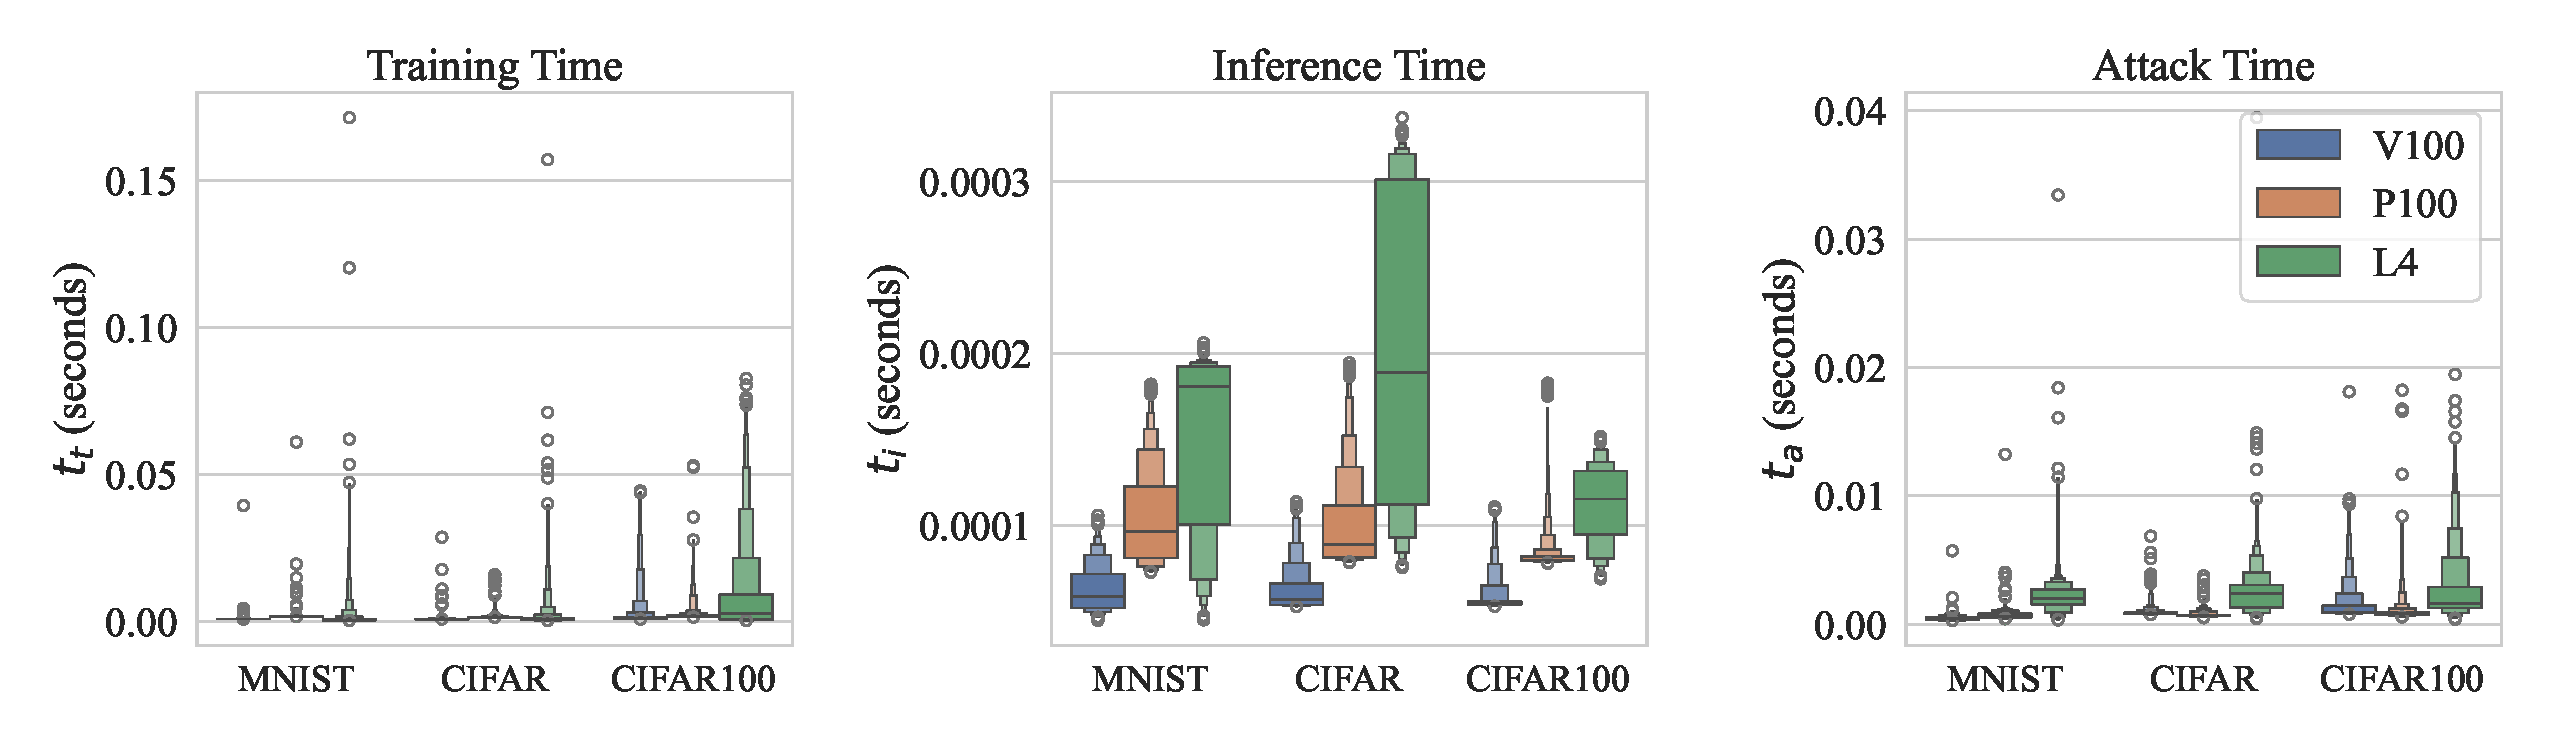
\includegraphics[width=\linewidth,clip]{plots/combined/time.pdf}
        \caption{Training (left), Prediction (center), and Attack (right) Times.}
        \label{fig:time}
    \end{subfigure}
    \begin{subfigure}[b]{.8\textwidth}
        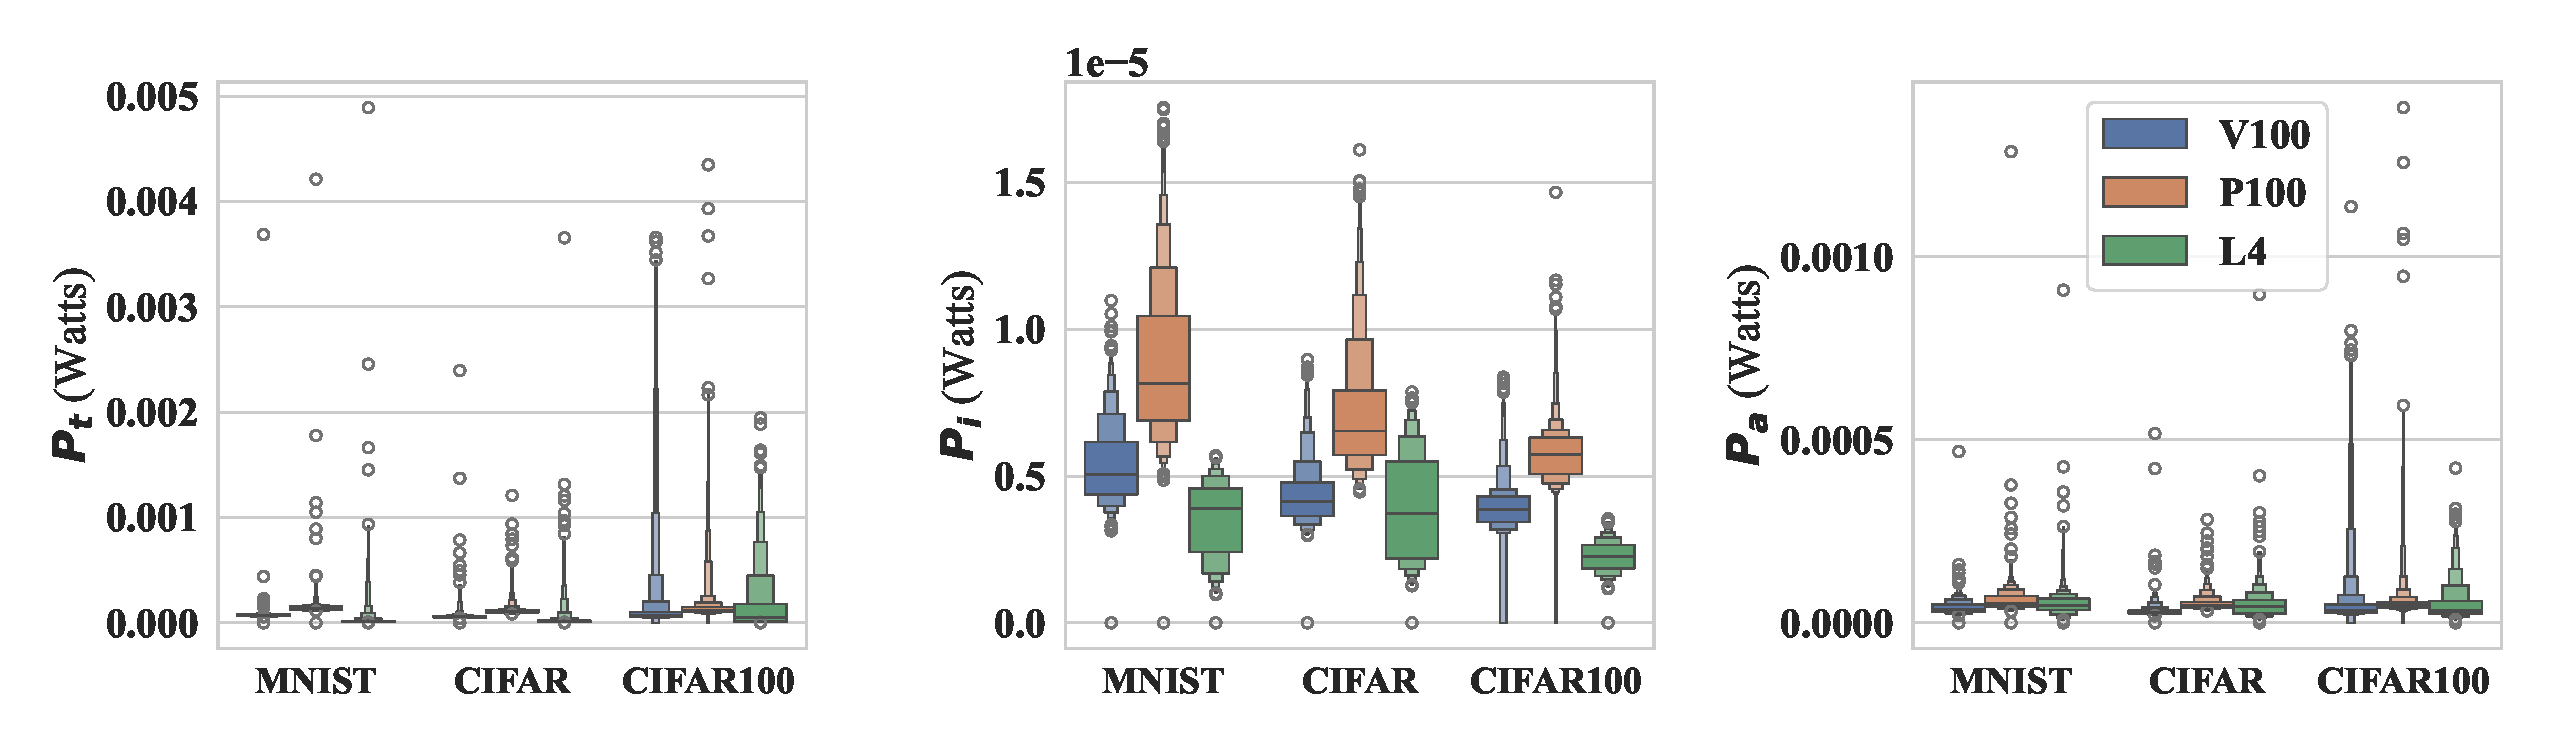
\includegraphics[width=\linewidth,clip]{plots/combined/power.pdf}
        \caption{Training (left), Prediction (center), and Attack (right) Power Consumption.}
        \label{fig:power}
    \end{subfigure}
    \begin{subfigure}[b]{.8\textwidth}
        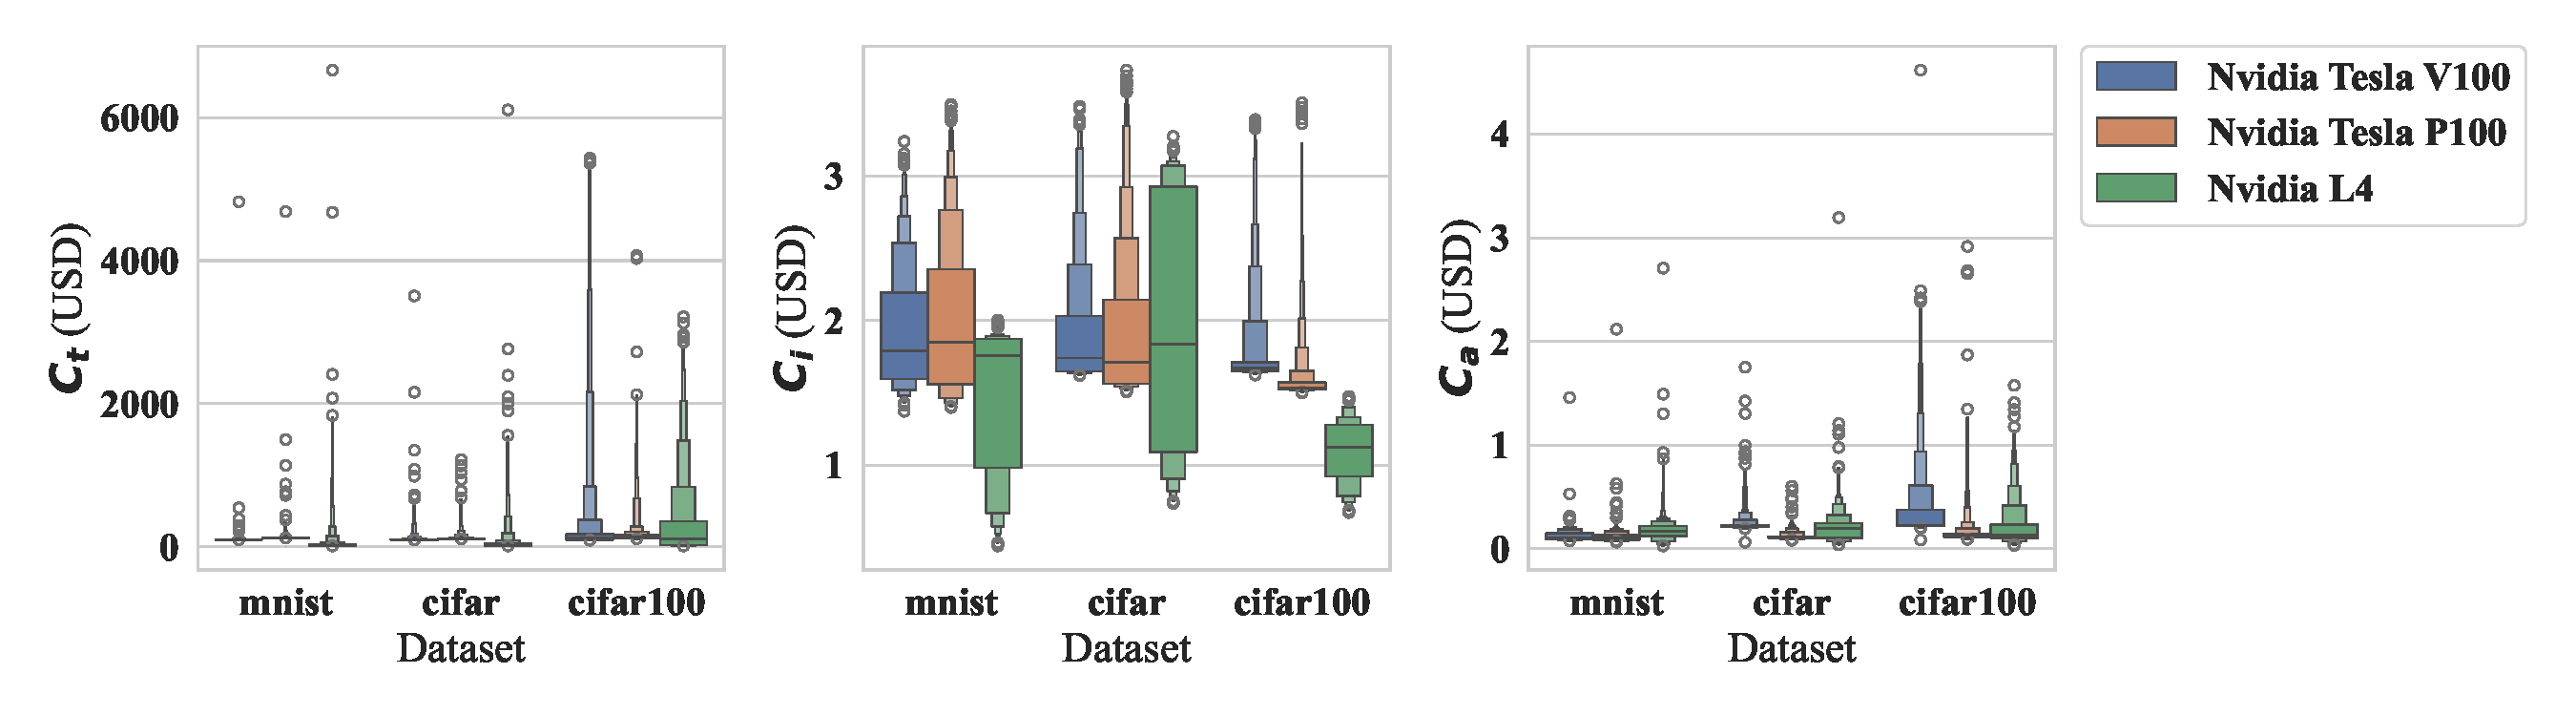
\includegraphics[width=\linewidth,clip]{plots/combined/cost.pdf}
        \caption{Training (left), Prediction (center), and Attack (right) Monetary Cost.}
        \label{fig:cost}
    \end{subfigure}
    \caption{This depicts the training, inference, and attack cost metrics for all hardware and datasets. For these plots, the y-axes have been scaled by the the number of samples for the sake of comparison.}
\end{figure*}


\subsection{Time, Power, Cost}
\label{res:cost}

Figure~\ref{fig:time} reveals the training time, inference time, and attack generation time across all datasets and models. Slower hardware (see Memory Bandwidth in Table~\ref{tab:hardware}) is only a few milliseconds slower, so this is unlikely to be noticeable to an end-user during inference. This should be no surprise since the less-capable hardware is meant to be used exclusively for inference. Additionally, the attack time (right sub-figure) increases with both the training (left) and prediction times (center) across hardware and datasets --- an expected result since this is driven by the number of samples and the inference time (see Eq.~\ref{attack_time}). We can also see that average training time per sample is takes slightly more than than attack generation time per sample (see:~\ref{fig:time} left and right plots).

The power consumption during training, inference, and attack generation for all hardware and datasets is illustrated in Figure~\ref{fig:power}. It tracks monetary cost (Figure~\ref{fig:cost}) closely, probably because that's the predominant cost for the datacenter itself~\cite{dayarathna2015data}, so it is unsurprising that cloud billing is correlated with the power requirement. Furthermore, we see that the largest dataset (CIFAR100) and smallest GPU (L4) require the least amount of power (Figure~\ref{fig:power}) for prediction, while differences between hardware and datasets are insignificant for the training and attack metrics. 

The monetary cost for each dataset and each piece of hardware is shown in Figure~\ref{fig:cost}. For all three datasets across all three pieces of hardware, the cost of training on a single sample often exceeds the cost of attacking a single sample. In the best case scenario, they are comparable, but attacks consistently succeed with only 100 samples (Figure~\ref{fig:acc}) while model training requires orders of magnitude more. 
%  However, we note that the attacker only needs to be lucky once, whereas the the model builder must be lucky always.

\begin{table*}
\centering
\caption{Comparison of AFR Models on the Combined dataset. The metrics are defined in Sec.~\ref{afr}}
\label{tab:combined}
\begin{tabular}{lrrrrrr}
\toprule
 & AIC & BIC & Concordance & Test Concordance & ICI & E50 \\
\midrule
Weibull & -5.57e+03 & -5.57e+03 & 0.84 & 0.84 & 0 & 0 \\
Log Logistic & -5.71e+03 & -5.71e+03 & 0.85 & 0.84 & 0.01 & 0 \\
Log Normal & -5.85e+03 & -5.85e+03 & 0.84 & 0.84 & 0.01 & 0 \\
\bottomrule
\end{tabular}
\end{table*}
  % Table II


\subsection{AFT Models}
\label{res:aft}

Table~\ref{tab:combined} shows the performance metrics for all three AFT models, as outlined in Section~\ref{survival_time}. A total 75\% of the available data were used to build the AFT models and 25\% were withheld for evaluation. The concordance is both strong ($>0.5$) and similar for all three AFT models and both the train and test sets. We observed no more than 1\% mean absolute error in the probabilities (ICI) and no error in the median probability (E50) across all three AFT models. Figure~\ref{fig:qq} depicts the observed and predicted probabilities for all three AFT models. For further analysis, we chose the Weibull AFT due to its superior fit in Figure~\ref{fig:qq}, and average test error of 1\% (ICI) and 0 error for the median sample (E50). We also see that these metrics are  functionally identical across all AFT models as well as between the test and train set of each model. 


Figure~\ref{fig:aft} shows the log-scale coefficients for the AFT model. It shows that epochs, batch size, and training time have no effect on the survival time. Additionally, the covariate value of 0 for random state indicates that random permutations of the training and test data have no effect on the survival time, which is expected. However, we can clearly see that inference time  is as strong an indicator as the attack noise distance, revealing that model speed is nearly as important as the the noise value of the attack ($\varepsilon$). Furthermore, we see that benign accuracy is negatively correlated with the survival time, confirming previous assertions that robustness ($S_{\theta}(t)$) is inversely related to benign accuracy (which is the standard indicator of generalization performance)~\cite{carlini_towards_2017}.

Using the $S_{\theta}(t)$ described in Section~\ref{aft}, we can model the effect of various hardware devices, which is depicted in Figure~\ref{fig:dummies}. It clearly shows that hardware choice has a relatively small effect (+/- 20\%) on robustness, despite the much larger disparity in cost outlined in Table~\ref{tab:hardware}.

\begin{figure*}[h!]
    \centering
    \captionsetup[subfigure]{skip=0pt} % Adjust the skip here
    \begin{subfigure}[b]{.3\linewidth}
        \centering
        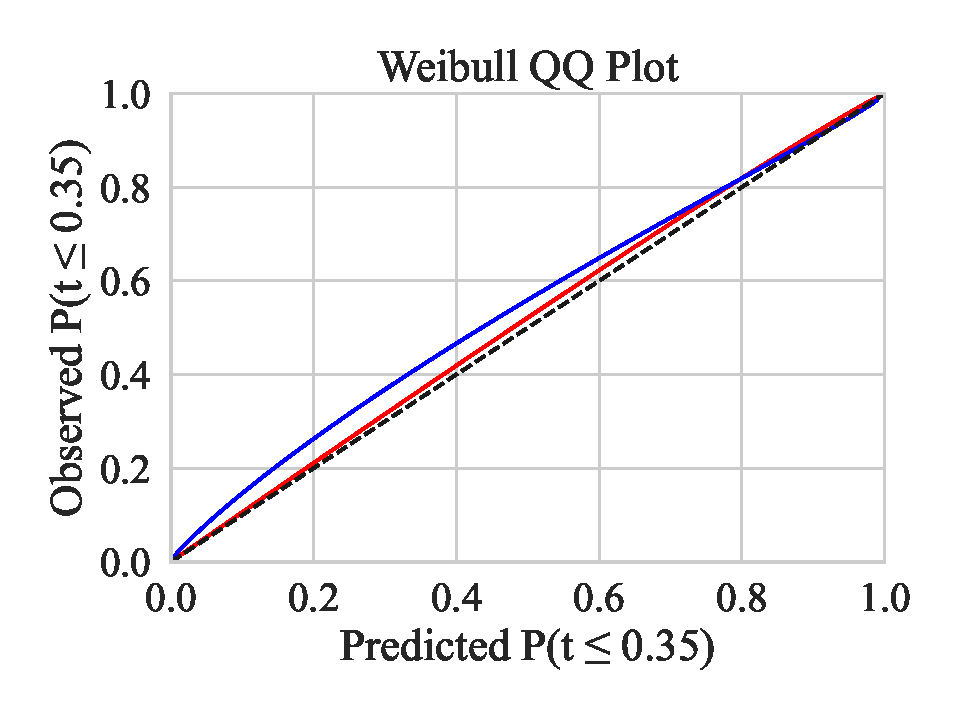
\includegraphics[width=\linewidth,clip]{plots/combined/weibull_qq.pdf}
        \caption{}
    \end{subfigure}
    \begin{subfigure}[b]{.3\linewidth}
        \centering
        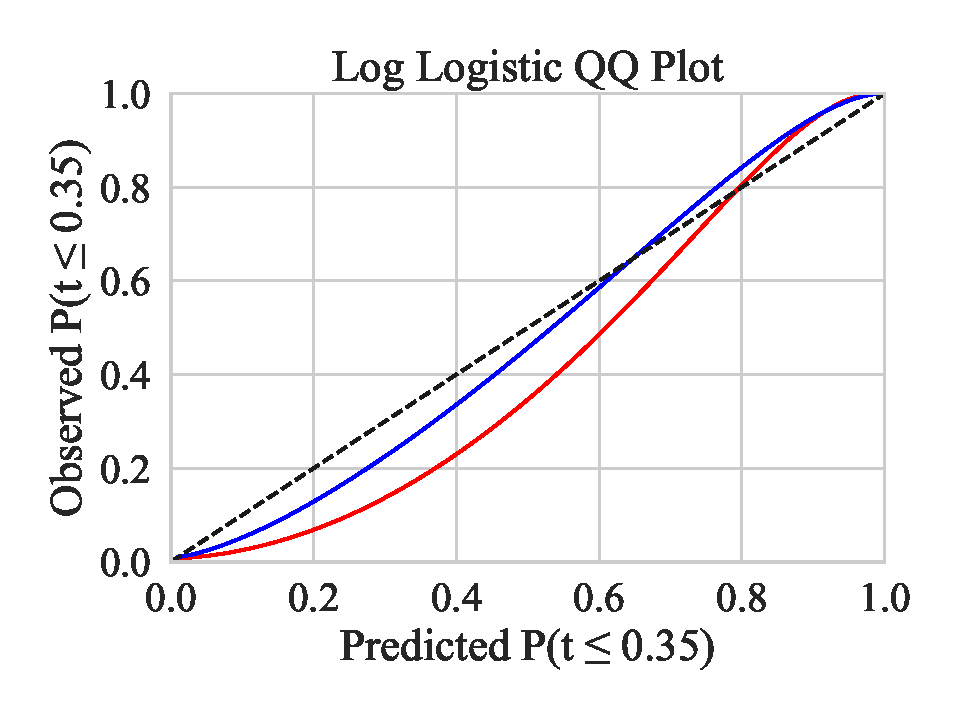
\includegraphics[width=\linewidth,clip]{plots/combined/log_logistic_qq.pdf}
        \caption{ }
    \end{subfigure}
    \begin{subfigure}[b]{.3\linewidth}
        \centering
        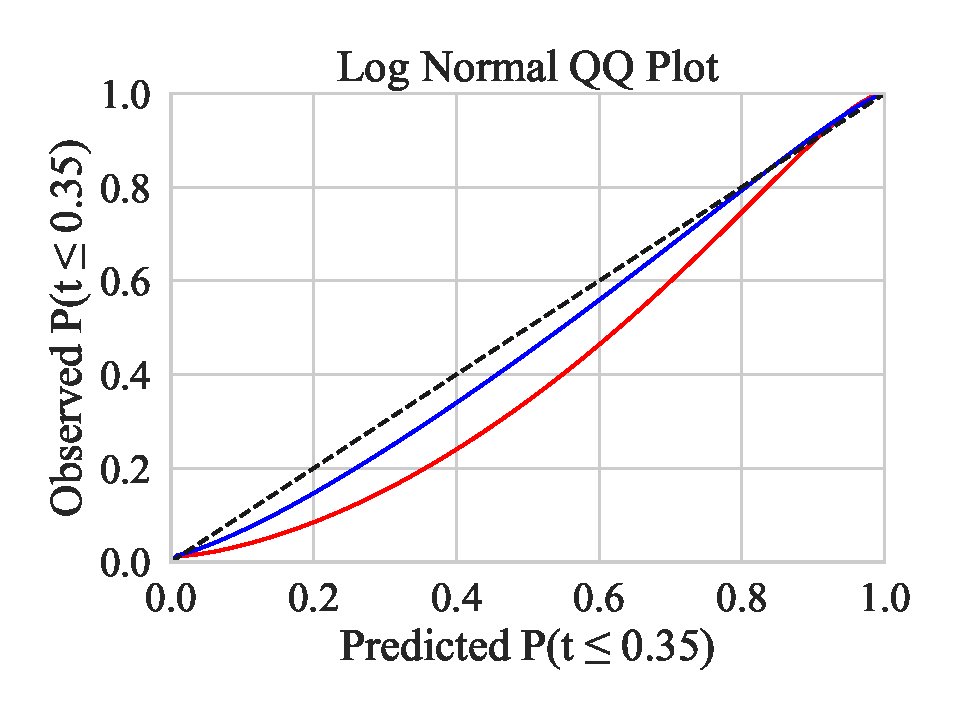
\includegraphics[width=\linewidth,clip]{plots/combined/log_normal_qq.pdf}
        \caption{}
    \end{subfigure}
    \caption{\cm{The red and blue lines depict the relationship between the modelled number of failures (x-axis) and the measured number of failures (y-axis) for the training set (blue) and test set (red). The dotted line indicates a perfect model.}}
    \label{fig:qq}
\end{figure*}
\begin{figure*}[h!]
    \centering
    \captionsetup[subfigure]{skip=0pt} % Adjust the skip here
    \begin{subfigure}{.5\linewidth}
        \centering
        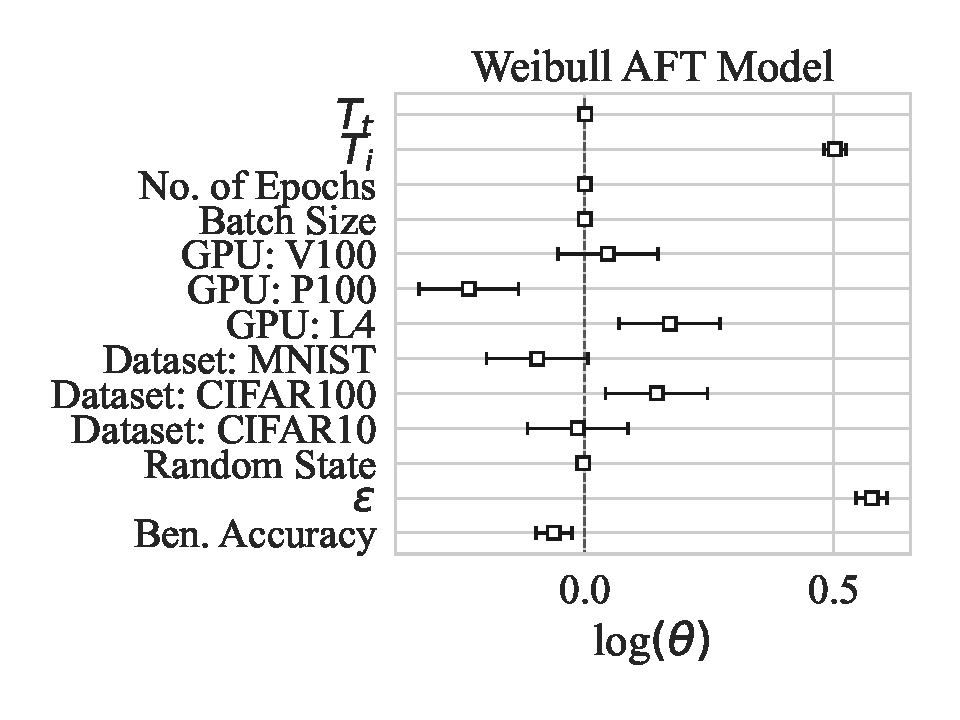
\includegraphics[width=\linewidth]{plots/combined/weibull_aft.pdf}
        \caption{Coefficients of the Covariates for the Weibull AFT model. Here, "Random State" is used as a control variable that should be (and is) close to 0.}
        \label{fig:aft}
    \end{subfigure}
    \begin{subfigure}[b]{.45\linewidth}
        \centering
        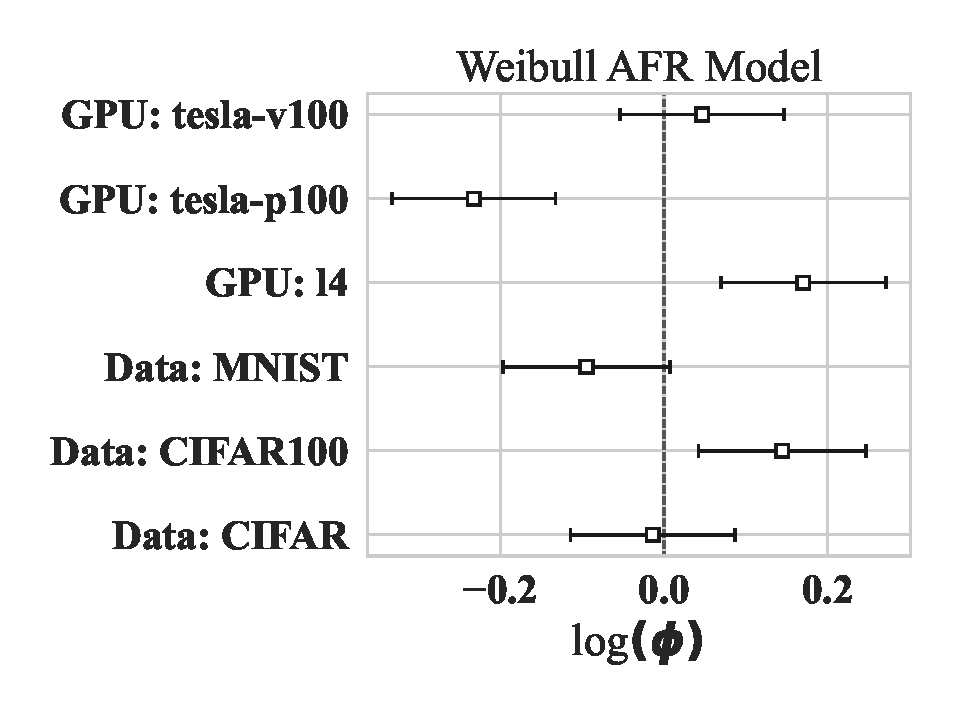
\includegraphics[width=\linewidth]{plots/combined/weibull_aft_dummies.pdf}
        \caption{AFT coefficients for devices and datasets on $S_{\theta}(t)$.}
        \label{fig:dummies}
    \end{subfigure}
    \caption{Weibull AFT Model.}
\end{figure*}


\subsection{Advantages of this Methodology}
\label{advantages}
\cm{Moved from the AFT section to here at Tommy's suggestion.}
\cm{The primary advantage of this methodology over the traditional test/train split measurements is that the precision of the latter is determined by the number of samples; whereas, the precision of the survival time estimate is driven by the resolution of our timing measurements. For test-set accuracy,  meeting the weakest safety-critical IEC standard (1 failure in a million) would require many millions of samples to confidently conclude that a model is safe. However, the presented AFT model has an average error rate of 1\% while requiring a very small number of samples (10 sets of 100) (see: Table~\ref{tab:combined}).}
Because of the small number of samples needed for building AFT models (when compared to testing against massive in-distribution test sets), AFT models could, for example, act as a unit test in machine learning applications. 
This is in contrast to a full-system integration tests to evaluate changes to a single model, signal processing technique, data storage format, or API access mechanism~\cite{schmoor2000sample,lachin1981introduction}. It could also be used to highlight error-prone classes or other subsets of data to reduce error or create synthetic samples as is common in medical research~\cite{kleinbaum1996survival}. Furthermore, by isolating changes and testing them as quickly as possible, it is easier to parse cause and effect when compared to full-system integration tests that could include many changes from many different development teams and require live and potentially dangerous systems (like cars, drones, or industrial equipment) to effectively test. To further increase development velocity, these models can quantify the marginal risk associated with each change, as dictated by the ISO 26262 standard~\cite{IEC61508}, allowing the model builder to make a quantitative assessment about the efficacy of a model change without testing the effect on real users. Additionally, since AFT models have strong predictive power for untested hyper-parameter combinations, this method has a potential to reduce the search space by quickly eliminating candidates that are unlikely to increase the survival time. 

\section{Considerations}
\label{considerations}

We have taken much care to conduct all timing measurements as carefully as possible.
Primarily, to minimize timing jitter and account for GPU parallelization, we assumed that the time-to-failure during the benign and adversarial accuracy measurements was uniform across the samples in each trial. 
While it is very possible (if not altogether guaranteed) that some classes or samples are easier to attack than others, we assume that this averages out over the 100 samples given to each attack. Further work examining, for example, the effect of imbalanced datasets on the the distribution of survival times across classes is outside the scope of this work, though the methodology would remain identical. Similarly, one could examine survival times for samples near the class boundary and compare them with prototypical samples near the center of the class cluster. 
However, given the strong results and uniformity across AFT functions in Table~\ref{tab:combined}, the uniform time assumption appears to be insignificant, though accounting for the failure rate per sample or class is likely to account for some of the remaining unexplained variance. 
Additionally, we chose a model and set of datasets small enough to fit entirely in GPU memory to minimize the confounding factors around parallelized, distributed, and/or federated learning as well as the complexities around storage hardware, file systems, and various access mechanisms. 
Larger models acting on larger datasets are likely to perform better on hardware with a higher GPU bandwidth, but the 48GB of VRAM provided by the L40 should be more than sufficient for vision tasks based on 8-bit images standard in the literature (e.g. MNIST, CIFAR10, CIFAR100). Furthermore, the attack batch size and the training batch size were set to be the same for every trial for each dataset and piece of hardware so that the attack timing would mimic the usage of regular users.
If anything, the smaller sample size of the attacks means that proportionally more parallelization overhead is needed per sample, leading to an underestimate of the attack efficacy compared to the benign measurements. Furthermore, while FGM is fast, it is not guaranteed to find failures as quickly as possible, meaning that the survival time estimate is likely to be overestimated.
In general, distributed/federated models were out of scope for this work, but architectural choices regarding the configuration of such methods could be evaluated using the cost and survival analysis techniques outlined above. 
The hyper-parameter search was restricted to only a single evasion attack (see Eq.~\ref{eq:fgm}) in the interest of time and budget, though this analysis would generalize to other evasion, extraction, inversion, or poisoning attacks~\cite{biggio_evasion_2013,biggio_poisoning_2013,choquette2021label,orekondy2019knockoff}. 


\section{Conclusions}
\label{conclusion}

In this work, we introduced survival analysis to machine learning, developed a method to quickly and efficiently test model parameter choices and evaluated them in the presence of adversarial noise, allowing one to the model performance as a function of tested model parameters.
Using this technique, it is clear that reduced run-times with newer and/or larger hardware, that adversarial robustness is not substantially effected and that the specific choice of attack parameters is far more important than model training time.
Furthermore, the data demonstrate the un-advertised training capability of the Nvidia L4 GPU which yields a 20\% increase in survival time while costing 75\% less than the V100 that's been typical in the literature over the last several years.

% no keywords
% For peer review papers, you can put extra information on the cover
% page as needed:
% \ifCLASSOPTIONpeerreview
% \begin{center} \bfseries EDICS Category: 3-BBND \end{center}
% \fi
%
% For peerreview papers, this IEEEtran command inserts a page break and
% creates the second title. It will be ignored for other modes.
\IEEEpeerreviewmaketitle

\clearpage
\bibliographystyle{IEEEtran}
\bibliography{bibliography}

\end{document}
